We live in a world in which information, data, is disseminated almost exclusively via the world wide web (WWW).  For researchers/practitioners in natural hazards engineering (NHE) that data is diverse, dynamic, distributed and often quite large. While manual gathering and processing of limited data sets is possible, the proliferation of data has overwhelmed the field of NHE greatly limiting its use. The SimCenter is releasing a series of applications that will enable researchers in field of natural hazards engineering (NHE) to incorporate these online resources in their numerical simulations through the use of scientific workflows: “scientific workflows are used to automate the analysis of data through multiple, distributed data resources in order to execute complex in silico experiments”.  [“Scientific workflows” paper by Katy Wolstencroft, Paul Fisher, David De Roure and Carole Goble.] The SimCenter is providing the NHE community with limited scientific workflow systems. Scientific Workflow Systems these are applications to build, launch, and monitor  scientific workflows. If one considers a scientific workflow as a sequence of applications being invoked akin to a jigsaw puzzle, as abstractly shown in \Cref{fig:jigsaw}, by providing applications to build. launch, and monitor scientific workflow, we mean an application that allows users to select from different applications for each jigsaw, then launch and monitor an application  which will run each application in the workflow passing the needed input and output data between the applications. The SimCenter systems are limited in that, unlike existing systems, limit the number and how the applications are put together.  

\begin{figure}[!htbp]
  \centering {
    
\includegraphics[width=0.75\textwidth]
    {images/jigsaw.png} }
  \caption{Abstraction of Scientific Workflow Application}
  \label{fig:jigsaw}
\end{figure}
 
Numerical simulations of real world phenonomena involve uncertainties and as a consequence need to generate measures of the uncertainty in the computed response. Those in NHE utilize a number of different uncertainty quantification (UW) methods, typically categorized into one of the following: 1) Forward methods, 2) Sensitivity methods,  and 3) Reliability methods.  All require that deterministic numerical simulations run repeatedly with different inputs. In SimCenter applications UQ engines, as shown in \Cref{fig:uqEngine},  run these simulations. The simulations can be run on either the user’s desktop computer or on high performance computers (HPC) made available to NHE community  through DesignSafe-ci.

 \begin{figure}[!htbp]
  \centering {
    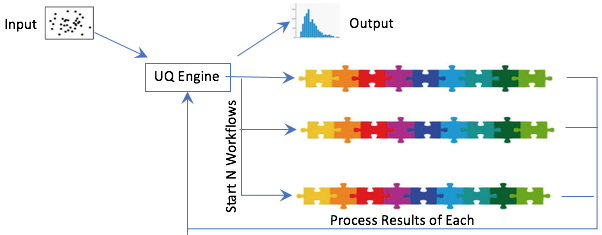
\includegraphics[width=0.75\textwidth]
    {images/uqEngine.png} }
  \caption{UQ Engine}
  \label{fig:uqEngine}
\end{figure}


The SimCenter is providing a number of scientific workflow  systems:  quoFEM, EE-UQ, WE-UQ, PBE, and RDT. Due to the limited programming resources available, these applications all are built using a common software framework. The framework, as shown in \Cref{fig:SimCenterSoftware}, comprises elements for Cloud Computing (limited to sending data and interfacing with remote service providers), UQ, SAM (structural analysis modeling), EVENT (earthquake, wind, tsunami, and storm surge), EDP (engineering demand parameters), FEM (finite element analysis and coupled Computational Fluid Dynamics-Finite Element Analysis), DL (damage and loss prediction). The framework also includes databases: DL( fragility curves for damage and loss calculations), Experimental and Simulation Models, and BE (built environment). In order to ingest data into the database BE is provided by software SimCEnter is developing as part of BRAILS.


\begin{figure}[!htbp]
  \centering {
    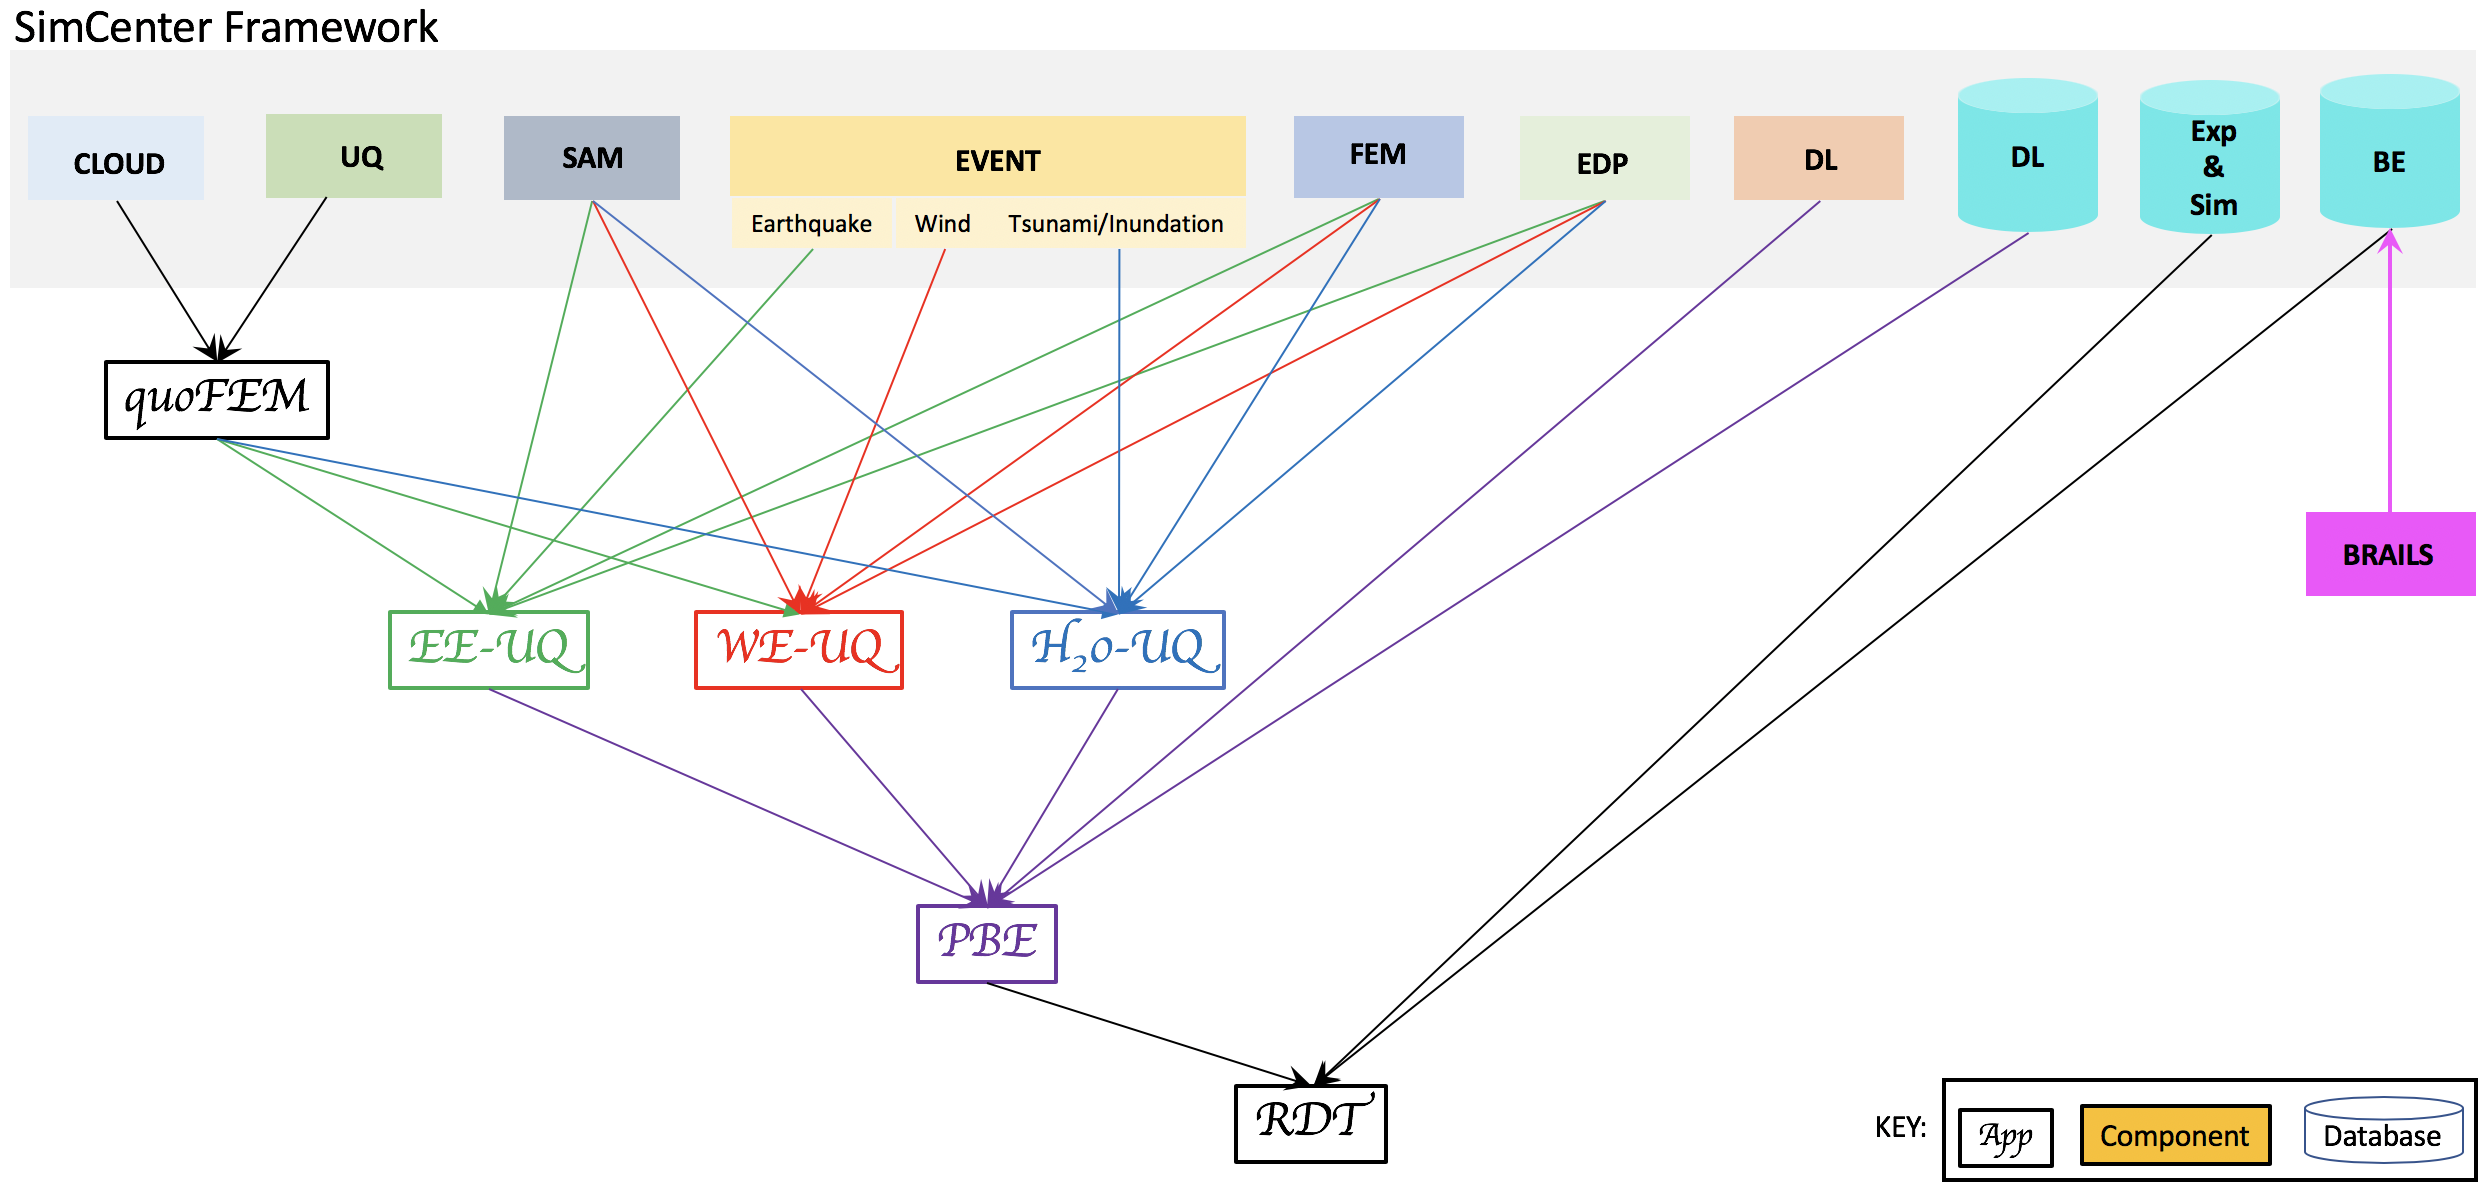
\includegraphics[width=0.75\textwidth]
    {images/SimCenterSoftware.png} }
  \caption{SimCenter Software Applications and Components}
  \label{fig:SimCenterSoftware}
\end{figure}

 This document outlines the software architecture behind the scientfic workflow systems  and the underlying framework.  These systems are made up of a number of containers, which themselves are made up of a number of components, which in turn are implemented by one or more classes. The architecture for released and planned SimCenter research applications is documented using the C4 model for visualizing the software architecture. A C4 model describes the software architecture in a series of diagrams with four levels of complexity:
\begin{enumerate}
\item A high level diagram showing how software system interacts with the world.
\item Diagrams showing the containers of the system.
\item Diagrams showing the components of each container.
\item Diagrams showing the how the components are built, class diagrams in object-oriented programs.
\end{enumerate}

This document is broken into a number of chapters. In the first we present the software architecture fo the applications EE-UQ, We-UQ, and PBE, which are applications for calculating response for a single structure. The architecture is also presented for RDT, an application for regional loss estimation. In the second we present the architecture behind applications used to generate information used in the regional loss estimation tool RDT. Finally a short descriotion of the versioing numbering employed by SimCenter for its applications. 

